Define the Hamiltonian in a second-quantized form and use this to compute the expectation value of the ground state (defining the so-called reference energy and later our Hartree-Fock functional) of
the helium atom.
Show that it is given by
\begin{equation}
    E[\Phi_0] = \expval{c}{\hat{H}}{c} = \sum_{i} \expval{i}{\hat{h}_0}{i} + \frac{1}{2} \sum_{ij} \left[\expval*{ij}{\frac{1}{r_{ij}}}{ij} - \expval*{ij}{\frac{1}{r_{ij}}}{ji}\right].
\end{equation}
Define properly the sums keeping in mind that the states $ij$ refer to all quantum numbers $n, l, m_l, s, m_s$.
Use the values for the various matrix elements listed at the end of the midterm to find the value of $E$ as function of $Z$ and compute $E$ as function of $Z$.

\subsection{}
We consider the Hamiltonian $\hat{H} = \hat{H}_0 + \hat{H}_I$, where $\hat{H}_0$ is the one-body part and $\hat{H}_I$ is the two-body part, given by
\begin{align*}
    \hat{H}_0 &= \sum_{i=1}^{N}\hat{h}_0(x_i), &
    \hat{H}_I &= \sum_{i<j}^{N}\frac{1}{r_{ij}}.
\end{align*}
In second quantization, we rewrite the one-body part as
\begin{equation}
    \hat{H}_0 = \sum_{\alpha\beta} \expval{\alpha}{\hat{h}_0}{\beta} a_\alpha^\dagger a_\beta.
\end{equation}
Then, the expectation value of the ground state with the one-body part is given by
\begin{equation*}
    \expval{\Phi_0}{\hat{H}_0}{\Phi_0} = \sum_{\alpha\beta} \expval{\alpha}{\hat{h}_0}{\beta} \expval{\Phi_0}{a_\alpha^\dagger a_\beta}{\Phi_0}.
\end{equation*}
For all states where either $\alpha > F, \beta > F$, we have that $\expval{\Phi_0}{a_\alpha^\dagger a_\beta}{\Phi_0} = 0$.
Thus, the sum is restricted to $i,j \le F$,
\begin{align*}
    \expval{\Phi_0}{\hat{H}_0}{\Phi_0} &= \sum_{ij} \expval{i}{\hat{h}_0}{j} \expval{\Phi_0}{a_i^\dagger a_j}{\Phi_0} \\
    &= \sum_{ij} \expval{i}{\hat{h}_0}{j} \delta_{ij} \\
    &= \sum_{i} \expval{i}{\hat{h}_0}{i},
\end{align*}
where we utilized the orthonormality of the single-particle states.

The two-body part is rewritten in second quantization as
\begin{equation*}
    \hat{H}_I = \frac{1}{2} \sum_{\alpha \beta \gamma \delta} \expval{\alpha \beta}{V}{\gamma \delta} a_\alpha^\dagger a_\beta^\dagger a_\delta a_\gamma.
\end{equation*}
The expectation value of the ground state with the two-body part is then
\begin{equation*}
    \expval{\Phi_0}{\hat{H}_I}{\Phi_0} = \frac{1}{2} \sum_{\alpha\beta\gamma\delta} \expval{\alpha\beta}{V}{\gamma\delta} \expval{\Phi_0}{a_\alpha^\dagger a_\beta^\dagger a_\delta a_\gamma}{\Phi_0}.
\end{equation*}
The possible contributing contractions are
\begin{align*}
    \wick{\c2 a_\alpha^\dagger \c1 a_\beta^\dagger \c1 a_\delta \c2 a_\gamma} &= \delta_{\alpha\gamma} \delta_{\beta\delta}, &
    \wick{\c1 a_\alpha^\dagger \c2 a_\beta^\dagger \c1 a_\delta \c2 a_\gamma} &= -\delta_{\alpha\delta} \delta_{\beta\gamma}. \\
\end{align*}
Whenever $\alpha > F$ or $\beta > F$, the expectation value vanishes, so we relabel the summation to $i, j$. The terms also vanish if $i = j$. % TODO: Reword maybe
We are then left with
\begin{equation*}
    \expval{\Phi_0}{\hat{H}_0}{\Phi_0} = \frac{1}{2} \sum_{\substack{ij \\ i \neq j}} \expval*{ij}{V}{ij} - \expval*{ij}{V}{ji}.
\end{equation*}

Gathering this, we get that the complete expectation value of the ground state is
\begin{equation}
    E[\Phi_0]
    = \expval{c}{\hat{H}}{c}
    = \sum_{i} \expval{i}{\hat{h}_0}{i} + \frac{1}{2} \sum_{\substack{ij \\ i \neq j}} \expval*{ij}{\frac{1}{r_{ij}}}{ij} - \expval*{ij}{\frac{1}{r_{ij}}}{ji},
\end{equation}
as we wanted to show.

In the case of the electrons in the helium atom, we only have $n = 1$, $l = 0$, differing only in the spin quantum number $m_s = \pm 1/2$.
The expectation value of the one-body part is then
\begin{equation*}
    \expval{\Phi_0}{\hat{h}_0}{\Phi_0} = \sum_{\sigma \in \{\pm 1/2\}} \expval{1\sigma}{\hat{h}_0}{1\sigma} = -\frac{Z^2}{n^2},
\end{equation*}
and the expectation value of the two-body part is, writing just $\sigma_{+}$ and $\sigma_{-}$ for the spins,
\begin{equation*}
    \expval{\Phi_0}{\hat{H}_I}{\Phi_0}
    = \frac{1}{2} \sum_{\substack{\sigma_{+}\sigma_{-}\\ \sigma_{+} \neq \sigma_{-}}}
    \underbrace{\expval*{\sigma_{+} \sigma_{-}}{\frac{1}{r_{\sigma_{+}\sigma_{-}}}}{\sigma_{+} \sigma_{-}}}_{\textnormal{Direct term}}
    - \underbrace{\expval*{\sigma_{+} \sigma_{-}}{\frac{1}{r_{\sigma_{+}\sigma_{-}}}}{\sigma_{-}\sigma_{+}}}_{\textnormal{Exchange term}}.
\end{equation*}
The exchange term vanishes since the states are orthogonal, and we are left with the direct term.
We are then just left with
\begin{equation*}
    \expval{\Phi_0}{\hat{H}_I}{\Phi_0} = \frac{1}{2}\left[ \expval*{\sigma_{+} \sigma_{-}}{\frac{1}{r_{\sigma_{+} \sigma_{-}}}}{\sigma_{+} \sigma_{-}} + \expval*{\sigma_{-} \sigma_{+}}{\frac{1}{r_{\sigma_{+} \sigma_{-}}}}{\sigma_{-} \sigma_{+}}\right].
\end{equation*}
As $\hat{H}_I$ is invariant under the change of label $\sigma$, we can simplify this to
\begin{equation*}
    \expval{\Phi_0}{\hat{H}_I}{\Phi_0} = \expval*{\sigma_{+} \sigma_{-}}{\frac{1}{r_{\sigma_{+} \sigma_{-}}}}{\sigma_{+} \sigma_{-}}.
\end{equation*}

Computing this, we find that the expectation value of the ground state is
\begin{equation}
    E[\Phi_0] = -Z^2 + \tfrac{5}{8}Z,
\end{equation}
which as a function of $Z$ is shown in \autoref{fig:energy}.

\begin{figure}[ht]
    \centering
    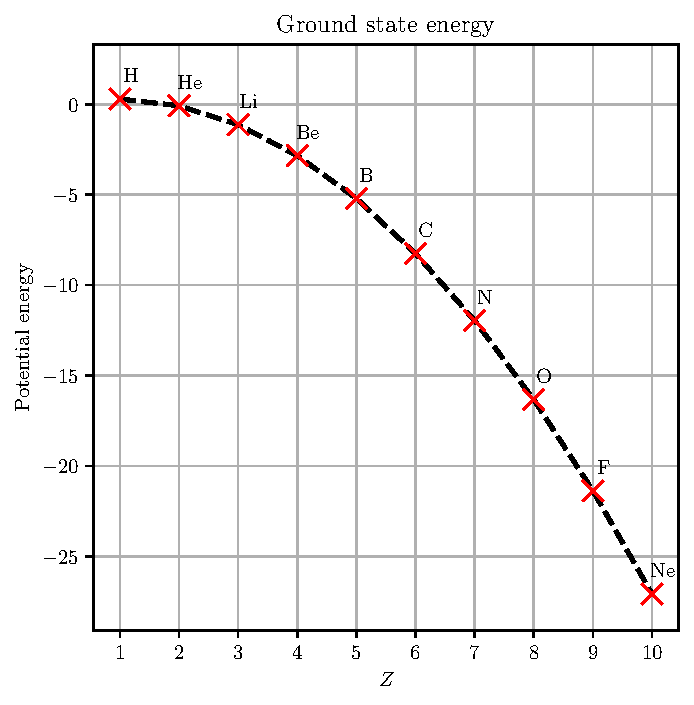
\includegraphics{figs/energy_plot.pdf}
    \caption{The expectation value of the ground states of an atom with two electrons as a function of the nuclear charge $Z$.\label{fig:energy}}
\end{figure}
